\subsection{Carry grips}


\subsubsection{Motivation}
At the end of the \preproject the sensor rig was possible to carry, but the grip was not very ergonomic.
Each hand had to hold each of the carbo fiber tubes to keep it balances, but this resulted in difficult handling, especially of the pitch angle.
Furthermore, the current design relies on controlling the software from a mobile phone, which requieres one hand in short perioeds of time, making the handling even more difficult.
To solve this problem, carry gimbal grips were designed and 3D printed.


\subsubsection{Base design}
Early on it was made clear that designing an ergonomic grip from scratch would be difficult and timeconsuming as it involves a lot of difficult geometric shapes.
Thus the idea was to use an existing design as a starting point.
To find a suitable design, the following search terms and model sites were used:

\begin{multicols}{2}
    \textbf{3Dmodel sites}:
    \begin{itemize}
        \item Thingiverse
        \item Printables
        \item GrapCad
        \item Cults
        \item Free3D
    \end{itemize}
    \columnbreak
    \textbf{Key words:}:
    \begin{itemize}
        \item handle
        \item grip
        \item ergonomic handle
        \item ergonomic grip
        \item carry handle
        \item carry grip
    \end{itemize}
\end{multicols}

A well designed set of ergonomic handles were found on Ptintables \cite{matulichErgonomicHandleBased}.
The design of the handles was well documented on the creators blog page \cite{matulichWhoseHandsAre2022}
It is based on the anatomy of the human hand and the selected model had the selected model had trochoidal finger grooves, making it a good starting point for the design of the carry grips.

As the model did however not fit my hands very well, so multiple iterations were made to find a good fit.
Firstly the rough scaling needed was found by printing the outline of the grip in multiple sizes.
This was donw in "vase mode", a method where the printer prints the outline of the model in one continous spiral, to make the iteration fast \cite{ghargeCuraVaseMode2022}. One of these test prinst is shown in figure \ref{fig:handle_iteration}.

After having figured out a rough size, the whole grip was printed in in a couple of different sizes and a blind test was performed on myself and a couple of friends to find the best fit.
With the eyes closed the test subjects were asked to hold different grips and say if it was too big or too small in any direction or if it felt okay.
The same grip were given to the test subjects multiple times to make sure the results were consistent.
Based on the results of this test, a final the final design is 10\% higher, 20\% wider and 25\% deeper than the original design.

\begin{figure}[H]
    \centering
    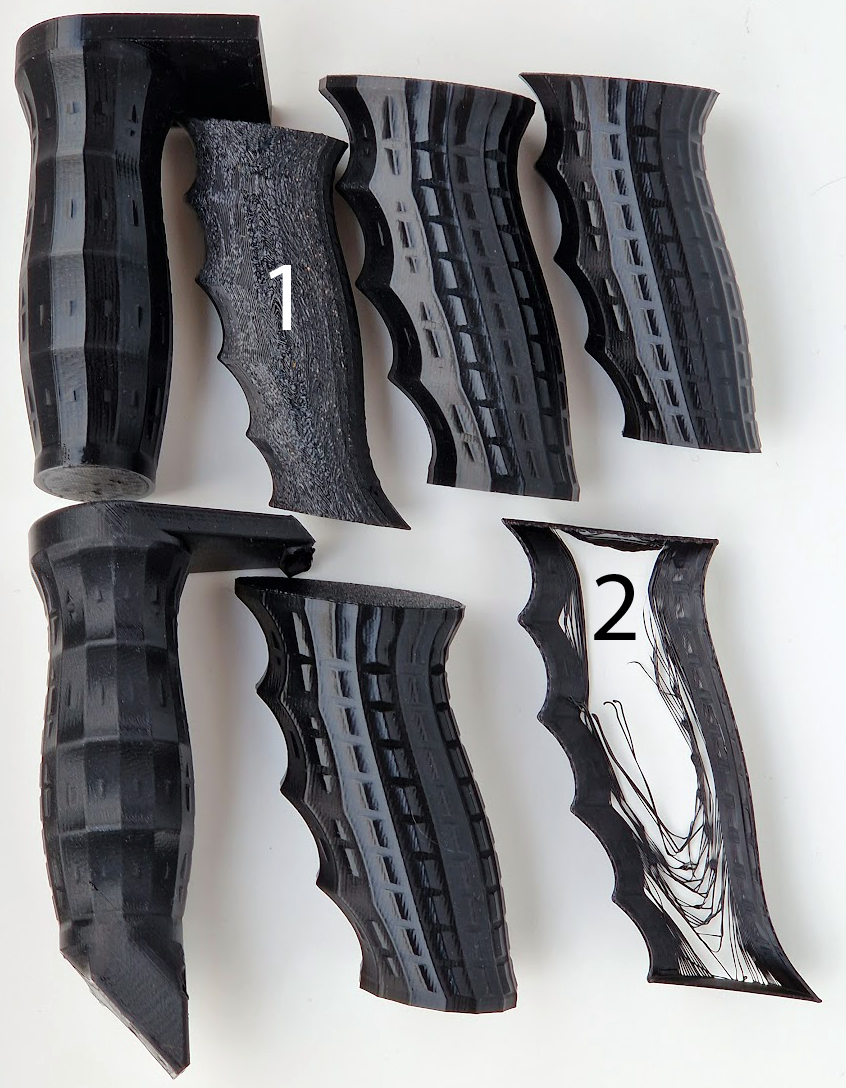
\includegraphics[width=.8\textwidth]{figures/3d_print/handles.png}
    \caption{Iterations on carry handle design. The handle marked with a 1 was printed sideways, resulting in a bad underside. The handle marked with a 2 shows one of the many handles printed in "vase mode" for fast iteration.}
    \label{fig:handle_iteration}
\end{figure}

\subsubsection{Integration with sensor rig}

\begin{figure}[H]
    \centering
    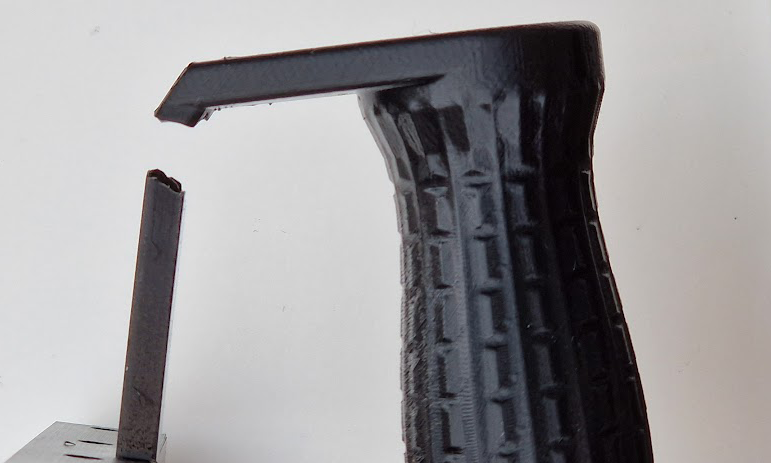
\includegraphics[width=\textwidth]{figures/3d_print/break.png}
    \caption{Some iterations on the camera mount design}
    \label{fig:hancle_break}
\end{figure}

\begin{figure}[H]
    \centering
    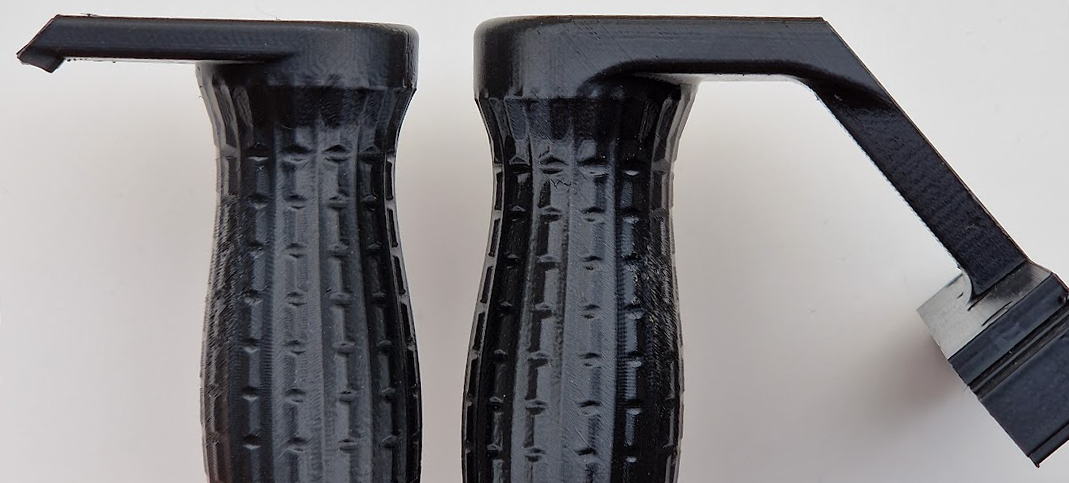
\includegraphics[width=\textwidth]{figures/3d_print/thickness.png}
    \caption{Some iterations on the camera mount design}
    \label{fig:handle_thickness}
\end{figure}